The accurate and efficient simulation of interface evolution is of fundamental importance in the simulation of multiphase flows. It is essential that the interface remains sharp. Large jumps of fluid density and viscosity across the interface should be correctly assumed by the numerical algorithm in order to satisfy the momentum balance at the vicinity of the interface.

Methods used to describe the evolution of interfaces can be clustered in two classes, namely: interface capturing and interface tracking methods. While in the former the interface is determined by an implicit function that is advected in a Eulerian frame (see Volume of Fluid \cite{VoF} and Level Set\cite{Osher01}), in the latter the interface evolution equation is solved in a Lagrangian fashion, for example by evolving marker particles. The spatial domain discretization using mesh and particles allows PFEM2 to select an appropriate combination of those approaches where the free position information is shared and interchanged by the particles and the fixed mesh.

There are several, but no large, differences between the PFEM-2 algorithm for homogeneous flows and the multi-fluids version. Those differences are produced by the density and viscosity discontinuities that appear in the fluid, consequently most of the changes are related to the strategies followed to capture correctly the interface between both fluids. Although some details presented in this section have been reported in \cite{Idelsohn13c}, however in this work we consider add important strategies that easily improve the accuracy and efficiency of the computation. 

Taking into account the Algorithm presented in section \ref{PFEM_Algorithm}, next are considerations to manage and improve each one of the stages for the particular case of multifluids problems. The following part is basically related with three aspects of the simulation: the kinematic treatment of the fluid particles during the X-IVAS stage, the pressure computation step and the enrichment technique for the free surface definition. Although these three topics are listed independently, the are closely related to each other during the computation and consequently the will be treated together in the next section.

\subsection{Internal interfaces tracking}

When 2 different fluids with free surface are considered, each particle carries the information of the fluid that was initially assigned, this quantity is represented by a scalar function $\lambda$ has integer values -1 or 1 depending if it belongs to the first or second fluid. This value is advected adding one equation to the \textit{Streamline Integration Stage}: $\frac{D\lambda}{Dt}=0$, i.e. each particle only keeps its marker value during the entire simulation. This function is projected to the mesh nodes to determine the free surface position. Mesh nodes consequently obtain real values from the projection different to the integer values $\pm1$ that particles transport. Free surface interface is defined as the set of points that satisfy the equation $\lambda=0$.

The last means, for instance, that even if a water particle is momentarily on an air regime, it will remain as a water particle for further determination of the interface position. However, in that case and because the most similar path to the real trajectory of the particle is desired, the particle leaves the streamlines and follows a trajectory defined by the acting forces, being the simplest one the parabolic motion (only gravity force) or coupled with a water droplet drag model.

After \textit{Projection Stage}, each node $j$ has a distance function-like value $\lambda_j$ which is used to determinate the instantaneous local interface inside each element. That zone is defined by an iso-line (an iso-plane in 3D) where $\lambda(\xx)=0$

%%HASTA ACA ESTA CHEQUEADO EL CAPITULO DE PFEM MULTIFLUIDS
\subsection{Shape function enrichments for pressure gradient discontinuity capturing}

In typical finite element methods, the gradient of the shape functions $\nabla\phi_j$ are continuous within each element, and therefore any unknown interpolated is also continuous. When the interface crosses an element the discontinuity in the material properties leads to discontinuities in the gradients of the unknowns that the interpolation used cannot capture. For the case of two different density fluids the interpolation errors in the pressure give rise to spurious velocities that can render the solution meaningless.

Enrichment methods add degrees of freedom at elements cut by the interface in order to reduce interpolation errors. In this work, the enriched space mainly used is based on the one presented by Coppola\cite{Coppola05}, which is illustrated in Figure \ref{fg:enrichment1}. The new degree of freedom could be statically condensed within each element in the pressure equation and then recovered in the correction step. Briefly, the way to construct the enrichment function $N^*$ is ensuring that $N^*(\xx_A)=1$ and $N^*(\xx_1)=N^*(\xx_2)=N^*(\xx_3)=0$.

Another set of enrichment functions is presented in Figure \ref{fg:enrichment2}, where, as in the previous case, the two new degrees of freedom can also be statically condensed. However, using this space it is possible to ensure continuity between elements, but paying the cost of having to rebuild the system matrix at each time step, which is an expensive task due to memory allocation.
This enrichment space is constructed following $N_A^*(\xx_A)=1$, $N_B^*(\xx_B)=1$ and $N_A^*(\xx_1)=N_A^*(\xx_2)=N_A^*(\xx_3)=N_A^*(\xx_B)=0$ and $N_B^*(\xx_1)=N_B^*(\xx_2)=N_B^*(\xx_3)=N_B^*(\xx_A)=0$ .

  \begin{figure}[H]
  \centering
    \subfloat[]{
	  \label{fg:enrichment1}         %% Etiqueta para la primera subfigura
	  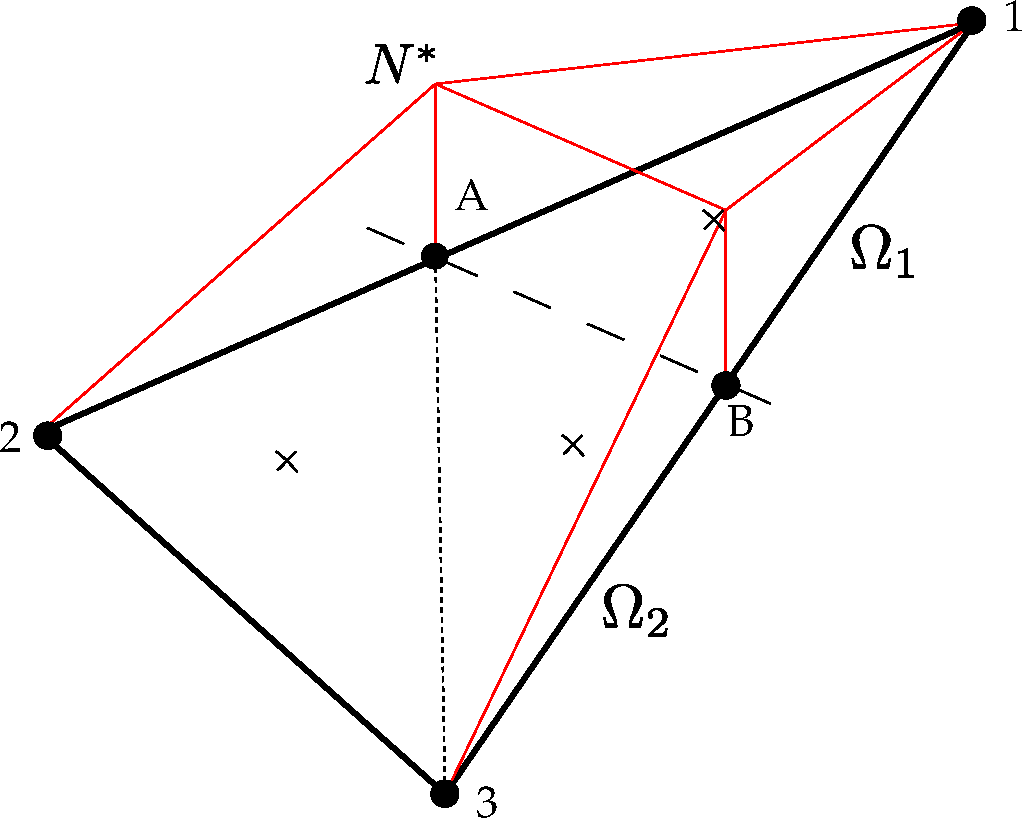
\includegraphics[width=.49\columnwidth]{images/enrichment1.pdf}
    }
    %%----segunda subfigura----
    \subfloat[]{
	  \label{fg:enrichment2}         %% Etiqueta para la segunda subfigura
	  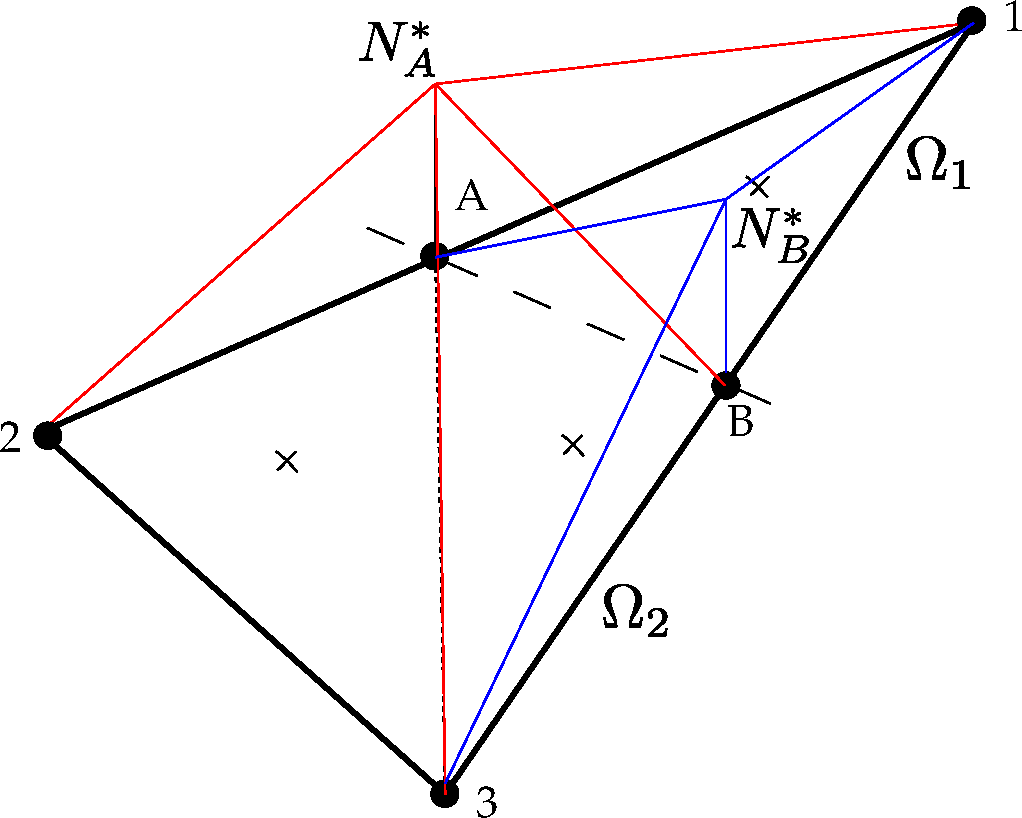
\includegraphics[width=.49\columnwidth]{images/enrichment2.pdf}
    }
   \caption{2D Enrichment functions. Figure \ref{fg:enrichment1} the enrichment proposed by Coppola and Figure \ref{fg:enrichment2} presents an enrichment space that can be used to ensure continuity between elements.}
   \label{fg:enrichment}                %% Etiqueta para la figura entera
\end{figure}

   Therefore, the pressure is now interpolated in the cut element following:

   \begin{equation}
      p_h(\xx) = \sum_{i=1}^{nnodes} (N_i(\xx) \ p_i) + N^*(\xx) \ p^*
   \end{equation}

   where $N_i$ are the traditional linear shape functions, and $N^*$ is defined as a linear combination of them (Equations \ref{N_enrichment-2} and \ref{N_enrichment-1}),

   \begin{align}
    N^*|_{\Omega_2} = & \ k_1 N_1 \label{N_enrichment-2}\\
    N^*|_{\Omega_1} = & \ k_2 N_2 + k_3 N_3 \label{N_enrichment-1}
   \end{align}
   where $k_1 = \dfrac{\psi_2-\psi_1}{\psi_2}$, $k_2 = \dfrac{\psi_1-\psi_2}{\psi_1}$ and $k_3 = -k_1\dfrac{\psi_3\psi_1}{\psi_3-\psi_1}$
	
	
   In order to capture the discontinuities and take advantage of the enrichment functions used, the integration rules need to be modified in elements cut by the front. The method we use is to divide each triangular element into up to three triangular sub elements. For each sub element the same integration rule as for the non-cut elements is used. Figure \ref{fg:enrichment}  shows that partition and the crosses represents the Gauss points for the integration. When using enrichment functions for the pressure, the material properties $\rho$,$\mu$ are taken as $\rho_1$,$\mu_1$ or $\rho_2$,$\mu_2$, depending on which part of the domain ($\Omega_1$ or $\Omega_2$) the integration point is found.

   \subsection{Pressure Iterations}

Most of multi-fluid flows present a large jump in the density properties, for instance water and air. For those cases, introducing a special strategy in the iterative algorithm to obtain acceptable convergence rates is mandatory. For instance, the strategy to introduce the last time step pressure field as the initial value for the first iteration of the next time step is not the best one. This is caused by the fact that the particles can move across several elements and through the interface during a time step (Figure 5.1) and, therefore, the pressure gradient of the previous time step would introduce a poor and even unstable approximation of the pressure forces.

Therefore, at each time-state, the value of the pressure is set to zero in order to avoid large errors in the evaluation of the pressure gradients in the initial value of the iterative process. As consequence of that, the acceleration over the particle only is due to viscous force and gravity force (pressure gradient is considered null) for this step.

    We are following the most similar path to the real trajectory of the particle. For the case of a water particle on water zones, we consider that the water streamlines are the best option. But on air zones, if the particle follows the air streamlines, poor approximations to the real trajectory will be obtained. Therefore, in the last situation, the water particle leaves the streamline and follows a trajectory defined by the acting forces, being the simplest one the parabolic motion (only gravity force) or coupled with a water droplet drag model.



\subsection{Pressure Stage}

  The Poisson equation for the pressure appears after applying the divergence operator to
  \begin{equation}
    \vv^{n+1}\  = \ \hat \vv^{n+1} - \dfrac{\Delta t}{\rho} \ [\nabla (\delta p)]^{n+1}
    \label{correction_cont}
  \end{equation}

  which remains
  \begin{equation}
   \dfrac{\Delta t}{\rho} \ \nabla \cdot [\nabla(\delta p^{n+1})] = \nabla \cdot \hat \vv_j^{n+1}
  \end{equation}

  integrating, weighting with local shape functions and weakening, we can obtain the elemental contribution
  \begin{equation}
   [\Delta t \int_{\Omega^e} \frac{1}{\rho} \nabla N^T \nabla N \ d\Omega] \delta p^{n+1} = [\int_{\Omega^e} \nabla N^T \phi \ d\Omega] \hat \vv_j^{n+1}
  \end{equation}

  The main advantage of the above proposed enrichment shape functions is that the added degree of freedom is local to the element cut by the interface and can therefore be condensed after the element matrix has been computed and before assembly.

  Therefore, if the element is not cut by the interface, the traditional lineal shape functions are used for weighting and the variables are approximated in terms of that space: $\delta p^{n+1}(\xx) = \sum_i N_i(\xx) \delta p^{n+1}_i$ and $\hat{\vv}^{n+1}(\xx) = \sum_i \phi_i(\xx) \hat{\vv}^{n+1}_i$, being $\phi_i = N_i$.

  On the other hand, if the element is cut by the interface, we choose $N = [N_1; N_2; N_3; N^*]$ as weight shape functions and to approximate the pressure field (keeping only the traditional shape functions $\phi = [N_1; N_2; N_3]$ to approximate the velocity field). Then, for the split elements, the system before the condensation is:

  \begin{equation*}
   \begin{pmatrix}
      L_{std} & L_{std}^*\\
      {L_{std}^*}^T & L^*
   \end{pmatrix}\;
    \begin{pmatrix}
      \delta p^{n+1}\\
      p^*
   \end{pmatrix}\; = \;
   \begin{pmatrix}
      D_{std}\\
      D^*
   \end{pmatrix}\;
   (\hat{\vv}^{n+1})
   \label{poisson}
\end{equation*}

where
\begin{itemize}
 \item ${(L_{std})}_{ij} = \Delta t \int_{\Omega^e} \dfrac{1}{\rho} \nabla N_i^T \nabla N_j \ d\Omega$ with $[i,j] = 1,2,3$ (size [$3$x$3$])
 \item ${(L_{std}^*)}_{i} = \Delta t \int_{\Omega^e} \dfrac{1}{\rho} \nabla N_i^T \nabla N^* \ d\Omega$ with $i = 1,2,3$ (size [$3$x$1$])
 \item $L^* = \Delta t \int_{\Omega^e} \dfrac{1}{\rho} \nabla {N^*}^T \nabla N^* \ d\Omega$ (size [$1$x$1$])
 \item ${(D_{std})}_{ij} = \int_{\Omega^e} \nabla N_i^T \phi_j \ d\Omega$ with $[i,j] = 1,2,3$ (size [$3$x$3$])
 \item ${(D^*)}_{j} = \int_{\Omega^e}  \nabla {N^*}^ \phi_j \ d\Omega$ with $j = 1,2,3$ (size [$1$x$3$])
\end{itemize}

  Therefore, the system is statically condensed obtaining:

  \begin{equation}
   [L_{std} - L_{std}^*\frac{1}{L^*}{L_{std}^*}^T](\delta p^{n+1}) = [D_{std}- L_{std}^*\frac{1}{L^*}D^*](\hat{\vv}^{n+1})
   \label{condensing}
  \end{equation}

  If we are interested in solving the system in absolute pressure terms, the final system is

  \begin{equation}
  [L_{std} - L_{std}^*\frac{1}{L^*}{L_{std}^*}^T](p^{n+1}) = [D_{std}- L_{std}^*\frac{1}{L^*}D^*](\hat{\vv}^{n+1}) + [L_{std} - L_{std}^*\frac{1}{L^*}{L_{std}^*}^T] (p^n)
   \label{condensing-abs}
  \end{equation}


\subsection{Correction Stage}

 This stage is typical from fractional steps. However, the new degree of freedom for the pressure, which was condensed previously, must be taken into account in this step to calculate the correct pressure gradient. Therefore, we must \textit{recover} $p^*$ doing:

  \begin{equation}
  {p^*}^{n+1} = \frac{1}{L^*}[D^* \hat{\vv}^{n+1} - {L_{std}^*}^Tp^{n+1} + {L_{std}^*}^Tp^{n} + L^*{p^*}^n]
  \label{recovering}
  \end{equation}

 Finally, the equation system presented in Equation \ref{correction} must be solved.

 \begin{equation}
  \int_{\Omega} N \rho \vv^{n+1} d\Omega = \int_{\Omega} N \rho \hat{\vv}^{n+1} d\Omega - \Delta t \ [\int_{\Omega} N_{std} \nabla p^{n+1} d\Omega + \int_{\Omega} N^* \nabla p* d\Omega]
  \label{correction}
 \end{equation}

 Besides the nodal velocity correction, it also must be done the correction over particles. Must be noted this correction is done projecting the variation of the nodal velocity.
	
  \begin{equation}
    \rho_p \vv_p^{n+1}\  = \ \rho_p \hat \vv_p^{n+1} - \boldsymbol{\pi}^{-1}(\delta \vv_j^{n+1})
    \label{correction_particles}
  \end{equation}
  where $\delta \vv_j^{n+1} = \vv_j^{n+1} - \hat \hat \vv_j^{n+1}$.


\subsection{Iterations to improve the pressure-velocity coupling}

The initial value of the pressure iterations is set to zero in order to avoid large errors in the evaluation of the pressure gradients in the initial value of the iterative process. It must be noticed that despite this first iteration of the pressure calculation is
of first order, further iterations improve the incompressibility of the solution. Doing this implies that the stabilization effect of the first order fractional step is lost due to the higher order scheme. Tests with hundreds of iterations were performed and, effectively,
spurious pressure oscillations appear in the solution. However, for practical applications, only two or three iterations are needed in order to obtain pressure convergence and, despite not being theoretically stable, pressure oscillations do not appear in the solution. For this reason no stabilization technique is required in this case.

Another justification because the pressure is restarted each time step is that we can not predict accurately the value of ${p^*}^n$ on Equation \ref{recovering} at the first iteration (using the latest $p^*$ of the previous time-step may introduce several problems due to the movement of the interface). Therefore, the acceleration for the velocity in X-IVAS only can have the viscous forces.

%Detalle del tema de la inicialización a cero de la presión, fundamentalmente por el hecho de que hay dos fluidos. Citar el clindro, como caso donde a pesar de haber un sólo fluido el algoritmo de puesta a cero de la presión sigue siendo válido.
